% Options for packages loaded elsewhere
\PassOptionsToPackage{unicode}{hyperref}
\PassOptionsToPackage{hyphens}{url}
%
\documentclass[
  ignorenonframetext,
]{beamer}
\usepackage{pgfpages}
\setbeamertemplate{caption}[numbered]
\setbeamertemplate{caption label separator}{: }
\setbeamercolor{caption name}{fg=normal text.fg}
\beamertemplatenavigationsymbolshorizontal
% Prevent slide breaks in the middle of a paragraph
\widowpenalties 1 10000
\raggedbottom
\setbeamertemplate{part page}{
  \centering
  \begin{beamercolorbox}[sep=16pt,center]{part title}
    \usebeamerfont{part title}\insertpart\par
  \end{beamercolorbox}
}
\setbeamertemplate{section page}{
  \centering
  \begin{beamercolorbox}[sep=12pt,center]{part title}
    \usebeamerfont{section title}\insertsection\par
  \end{beamercolorbox}
}
\setbeamertemplate{subsection page}{
  \centering
  \begin{beamercolorbox}[sep=8pt,center]{part title}
    \usebeamerfont{subsection title}\insertsubsection\par
  \end{beamercolorbox}
}
\AtBeginPart{
  \frame{\partpage}
}
\AtBeginSection{
  \ifbibliography
  \else
    \frame{\sectionpage}
  \fi
}
\AtBeginSubsection{
  \frame{\subsectionpage}
}

\usepackage{amsmath,amssymb}
\usepackage{iftex}
\ifPDFTeX
  \usepackage[T1]{fontenc}
  \usepackage[utf8]{inputenc}
  \usepackage{textcomp} % provide euro and other symbols
\else % if luatex or xetex
  \usepackage{unicode-math}
  \defaultfontfeatures{Scale=MatchLowercase}
  \defaultfontfeatures[\rmfamily]{Ligatures=TeX,Scale=1}
\fi
\usepackage{lmodern}
\usetheme[]{default}
\ifPDFTeX\else  
    % xetex/luatex font selection
\fi
% Use upquote if available, for straight quotes in verbatim environments
\IfFileExists{upquote.sty}{\usepackage{upquote}}{}
\IfFileExists{microtype.sty}{% use microtype if available
  \usepackage[]{microtype}
  \UseMicrotypeSet[protrusion]{basicmath} % disable protrusion for tt fonts
}{}
\makeatletter
\@ifundefined{KOMAClassName}{% if non-KOMA class
  \IfFileExists{parskip.sty}{%
    \usepackage{parskip}
  }{% else
    \setlength{\parindent}{0pt}
    \setlength{\parskip}{6pt plus 2pt minus 1pt}}
}{% if KOMA class
  \KOMAoptions{parskip=half}}
\makeatother
\usepackage{xcolor}
\newif\ifbibliography
\setlength{\emergencystretch}{3em} % prevent overfull lines
\setcounter{secnumdepth}{-\maxdimen} % remove section numbering


\providecommand{\tightlist}{%
  \setlength{\itemsep}{0pt}\setlength{\parskip}{0pt}}\usepackage{longtable,booktabs,array}
\usepackage{calc} % for calculating minipage widths
\usepackage{caption}
% Make caption package work with longtable
\makeatletter
\def\fnum@table{\tablename~\thetable}
\makeatother
\usepackage{graphicx}
\makeatletter
\def\maxwidth{\ifdim\Gin@nat@width>\linewidth\linewidth\else\Gin@nat@width\fi}
\def\maxheight{\ifdim\Gin@nat@height>\textheight\textheight\else\Gin@nat@height\fi}
\makeatother
% Scale images if necessary, so that they will not overflow the page
% margins by default, and it is still possible to overwrite the defaults
% using explicit options in \includegraphics[width, height, ...]{}
\setkeys{Gin}{width=\maxwidth,height=\maxheight,keepaspectratio}
% Set default figure placement to htbp
\makeatletter
\def\fps@figure{htbp}
\makeatother

\usepackage{booktabs}
\usepackage{longtable}
\usepackage{array}
\usepackage{multirow}
\usepackage{wrapfig}
\usepackage{float}
\usepackage{colortbl}
\usepackage{pdflscape}
\usepackage{tabu}
\usepackage{threeparttable}
\usepackage{threeparttablex}
\usepackage[normalem]{ulem}
\usepackage{makecell}
\usepackage{xcolor}
\newcommand{\theHtable}{\thetable}
\makeatletter
\@ifpackageloaded{tcolorbox}{}{\usepackage[skins,breakable]{tcolorbox}}
\@ifpackageloaded{fontawesome5}{}{\usepackage{fontawesome5}}
\definecolor{quarto-callout-color}{HTML}{909090}
\definecolor{quarto-callout-note-color}{HTML}{0758E5}
\definecolor{quarto-callout-important-color}{HTML}{CC1914}
\definecolor{quarto-callout-warning-color}{HTML}{EB9113}
\definecolor{quarto-callout-tip-color}{HTML}{00A047}
\definecolor{quarto-callout-caution-color}{HTML}{FC5300}
\definecolor{quarto-callout-color-frame}{HTML}{acacac}
\definecolor{quarto-callout-note-color-frame}{HTML}{4582ec}
\definecolor{quarto-callout-important-color-frame}{HTML}{d9534f}
\definecolor{quarto-callout-warning-color-frame}{HTML}{f0ad4e}
\definecolor{quarto-callout-tip-color-frame}{HTML}{02b875}
\definecolor{quarto-callout-caution-color-frame}{HTML}{fd7e14}
\makeatother
\makeatletter
\@ifpackageloaded{caption}{}{\usepackage{caption}}
\AtBeginDocument{%
\ifdefined\contentsname
  \renewcommand*\contentsname{Table of contents}
\else
  \newcommand\contentsname{Table of contents}
\fi
\ifdefined\listfigurename
  \renewcommand*\listfigurename{List of Figures}
\else
  \newcommand\listfigurename{List of Figures}
\fi
\ifdefined\listtablename
  \renewcommand*\listtablename{List of Tables}
\else
  \newcommand\listtablename{List of Tables}
\fi
\ifdefined\figurename
  \renewcommand*\figurename{Figure}
\else
  \newcommand\figurename{Figure}
\fi
\ifdefined\tablename
  \renewcommand*\tablename{Table}
\else
  \newcommand\tablename{Table}
\fi
}
\@ifpackageloaded{float}{}{\usepackage{float}}
\floatstyle{ruled}
\@ifundefined{c@chapter}{\newfloat{codelisting}{h}{lop}}{\newfloat{codelisting}{h}{lop}[chapter]}
\floatname{codelisting}{Listing}
\newcommand*\listoflistings{\listof{codelisting}{List of Listings}}
\makeatother
\makeatletter
\makeatother
\makeatletter
\@ifpackageloaded{caption}{}{\usepackage{caption}}
\@ifpackageloaded{subcaption}{}{\usepackage{subcaption}}
\makeatother
\ifLuaTeX
  \usepackage{selnolig}  % disable illegal ligatures
\fi
\usepackage{bookmark}

\IfFileExists{xurl.sty}{\usepackage{xurl}}{} % add URL line breaks if available
\urlstyle{same} % disable monospaced font for URLs
\hypersetup{
  pdftitle={Class 09},
  pdfauthor={Sarah E. Grabinski},
  hidelinks,
  pdfcreator={LaTeX via pandoc}}

\title{Class 09}
\subtitle{DATA1220-55, Fall 2024}
\author{Sarah E. Grabinski}
\date{2024-09-18}

\begin{document}
\frame{\titlepage}

\begin{frame}[fragile]{Homework 2}
\phantomsection\label{homework-2}
\begin{itemize}
\item
  \href{https://canvas.jcu.edu/files/3708401/download?download_frd=1}{Instructions}
  (\texttt{homework2\_instructions.pdf}), a
  \href{https://canvas.jcu.edu/files/3708307/download?download_frd=1}{Quarto
  markdown template} (\texttt{homework2\_template.qmd}), and an
  \href{https://canvas.jcu.edu/files/3708306/download?download_frd=1}{example
  HTML output} (\texttt{homework2\_example.html}) are available for
  download under Chapter 2 on the
  \href{https://canvas.jcu.edu/courses/36290/modules}{Modules} page in
  Canvas.
\item
  Upload \textbf{\emph{TWO}} (2) documents to
  \href{https://canvas.jcu.edu/courses/36290/assignments/451733}{Homework
  2} on the
  \href{https://canvas.jcu.edu/courses/36290/assignments}{Assignments}
  page in Canvas by Friday 9/20/2024 by 6:00pm:
  \texttt{homework2\_yourlastname.qmd} and
  \texttt{homework2\_yourlastname.html}
\item
  \href{https://canvas.jcu.edu/files/3708369/download?download_frd=1}{Video
  walk-through} of Homework 2 under Tutorials on the Modules page in
  Canvas. Make sure you're caught up on the
  \href{https://canvas.jcu.edu/files/3695568/download?download_frd=1}{video
  walk-through of homework 1}.
\end{itemize}
\end{frame}

\begin{frame}{Late Policy}
\phantomsection\label{late-policy}
``This homework is due by 6:00pm on Friday, 9/20/24. No credit will be
lost for assignments received by 7:00pm to account for issues with
uploading. 10\% of the points will be deducted from assignments received
by 9:00am on Saturday, 9/21/24. Assignments turned in after this point
are only eligible for 50\% credit, so it benefits you to turn in
whatever you have completed by the due date.''
\end{frame}

\begin{frame}{How can I get help with homework?}
\phantomsection\label{how-can-i-get-help-with-homework}
\begin{itemize}
\item
  \textbf{Read the
  \href{https://canvas.jcu.edu/files/3669904/download?download_frd=1}{textbook}.}
  Many of you are asking for additional examples. Luckily, there are
  tons we didn't go over in the textbook.
\item
  \textbf{Look at the
  \href{https://canvas.jcu.edu/courses/36290/assignments/451733}{homework}
  early}. Only 1 person has looked at the homework since I posted it.
  Make sure you leave enough time to get help if you need it.
\item
  \textbf{Ask a question on our
  \href{https://campuswire.com/c/G6427C531/feed}{Campuswire class
  feed}.} I'm only one person, and I may not be able to give you a
  prompt answer. However, the 20+ other people in the class might be
  able to.
\item
  \textbf{Come to office hours.} I will be available after class today
  Wednesday 9/25/2024 from 2:30pm - 4:00pm. If you cannot make it, reach
  out to me to try and schedule an appointment.
\end{itemize}
\end{frame}

\begin{frame}{Chapter 3 Objectives}
\phantomsection\label{chapter-3-objectives}
\begin{itemize}
\item
  Define probability, random processes, and the law of large numbers
\item
  Describe the sample space for disjoint and non-disjoint outcomes
\item
  Calculate probabilities using the General Addition and Multiplication
  Rules
\item
  Create a probability distribution for disjoint outcomes
\end{itemize}
\end{frame}

\begin{frame}{Defining Probability}
\phantomsection\label{defining-probability}
What does the word \textbf{probability} mean to you?

\pause

``Highly likely''

\pause

``Probably''

\pause

``About even''

\pause

``Almost no chance''
\end{frame}

\begin{frame}{People interpret probability differently}
\phantomsection\label{people-interpret-probability-differently}
\begin{figure}[H]

{\centering \includegraphics{class09_files/mediabag/perceptions-of-proba.png}

}

\caption{Did your estimate fall within these ranges? Are these ranges
reasonable?}

\end{figure}%
\end{frame}

\begin{frame}{So what is probability?}
\phantomsection\label{so-what-is-probability}
\begin{tcolorbox}[enhanced jigsaw, title=\textcolor{quarto-callout-note-color}{\faInfo}\hspace{0.5em}{Frequentist Definition}, opacitybacktitle=0.6, opacityback=0, colbacktitle=quarto-callout-note-color!10!white, colframe=quarto-callout-note-color-frame, colback=white, leftrule=.75mm, breakable, toprule=.15mm, titlerule=0mm, left=2mm, coltitle=black, arc=.35mm, bottomtitle=1mm, toptitle=1mm, rightrule=.15mm, bottomrule=.15mm]

The proportion of times that a particular outcome would occur if we
observed a random process an infinite number of times.

\end{tcolorbox}

\begin{itemize}
\item
  A \textbf{random process} is one where you know which outcomes are
  possible (i.e.~the \textbf{sample space}) but you don't know which
  outcome comes next
\item
  Examples of a \textbf{random process}: coin toss, die roll, stock
  market
\end{itemize}
\end{frame}

\begin{frame}{How do you know a process is random?}
\phantomsection\label{how-do-you-know-a-process-is-random}
\begin{figure}[H]

{\centering 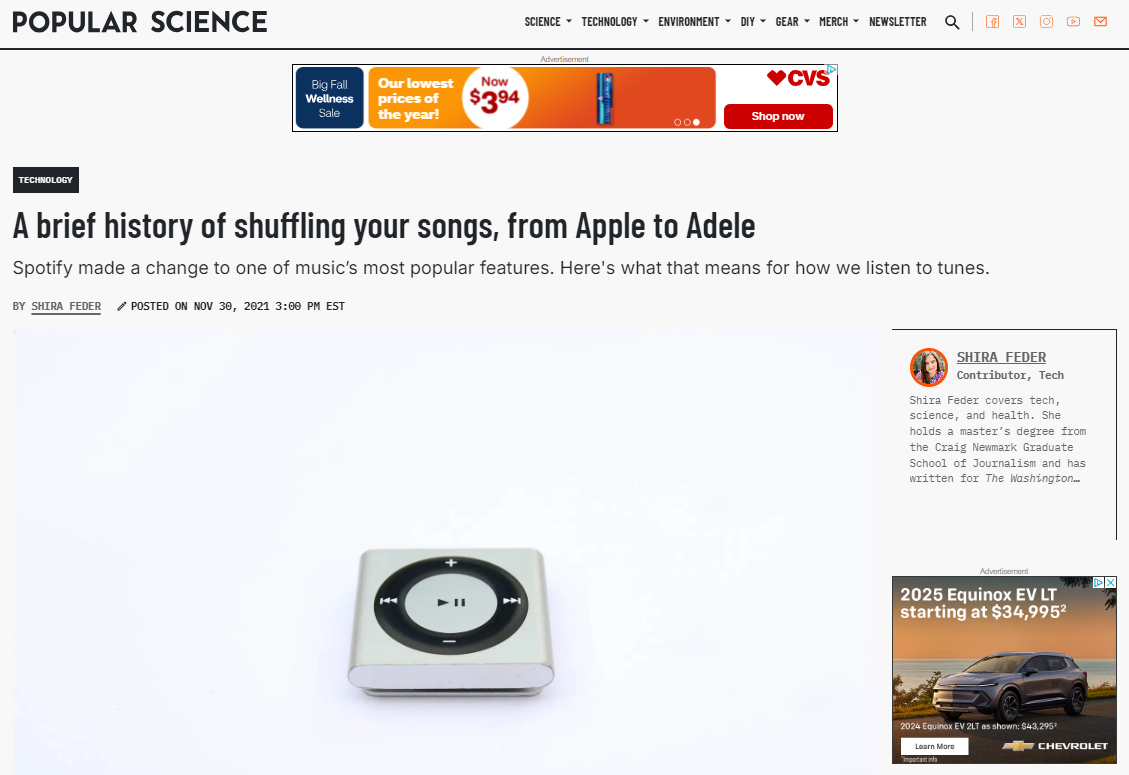
\includegraphics{class09_files/mediabag/shuffle.png}

}

\caption{Both Apple and Spotify took steps to make their ``shuffle''
features less random after complaints from users.}

\end{figure}%
\end{frame}

\begin{frame}{A brief history of ``Shuffle''}
\phantomsection\label{a-brief-history-of-shuffle}
\begin{itemize}
\item
  January 11, 2005 -- Apple releases the iPod Shuffle, a small device
  capable only of playing music randomly (``true'' shuffle)
\item
  September 7, 2005 -- Apple offers ``Smart Shuffle'' in response to
  complaints, which controlled how likely songs from the same album or
  artist would play close together
\item
  July 2011 -- Spotify launches in the United States using the
  \href{https://engineering.atspotify.com/2014/02/28/how-to-shuffle-songs/}{Fisher-Yates
  Algorithm}, which is like picking tickets out of a hat until no more
  remain
\item
  February 2014 -- Spotify modifies their sampling algorithm to ensure
  an even distribution across albums/artists
\end{itemize}
\end{frame}

\begin{frame}{What went wrong?}
\phantomsection\label{what-went-wrong}
\begin{itemize}
\item
  The human brain is good at finding patterns in noise, even when there
  are none
\item
  If an artist is repeated ``too soon'', the listener doesn't feel the
  order is random
\item
  We perceive a ``random'' distribution as also being ``uniform'' and
  ``fair''
\end{itemize}
\end{frame}

\begin{frame}{So why didn't we like a ``true'' random shuffle?}
\phantomsection\label{so-why-didnt-we-like-a-true-random-shuffle}
\begin{itemize}
\item
  Songs not evenly distributed across albums and artists on a playlist
\item
  Some albums/artists may play more frequently than others simply
  because they have more songs in the library/on the playlist
\item
  Each song is equally likely to play next, but not each artist
\item
  Artists/albums with more songs also more likely to play in a row
\item
  A true random shuffle might play the same artist multiple times in a
  row
\item
  It's unusual but not impossible to roll a 1 on a die 3 times in a row
\item
  It's also possible for the same song to play twice in a row
\end{itemize}
\end{frame}

\begin{frame}{Example: Spotify Playlists}
\phantomsection\label{example-spotify-playlists}
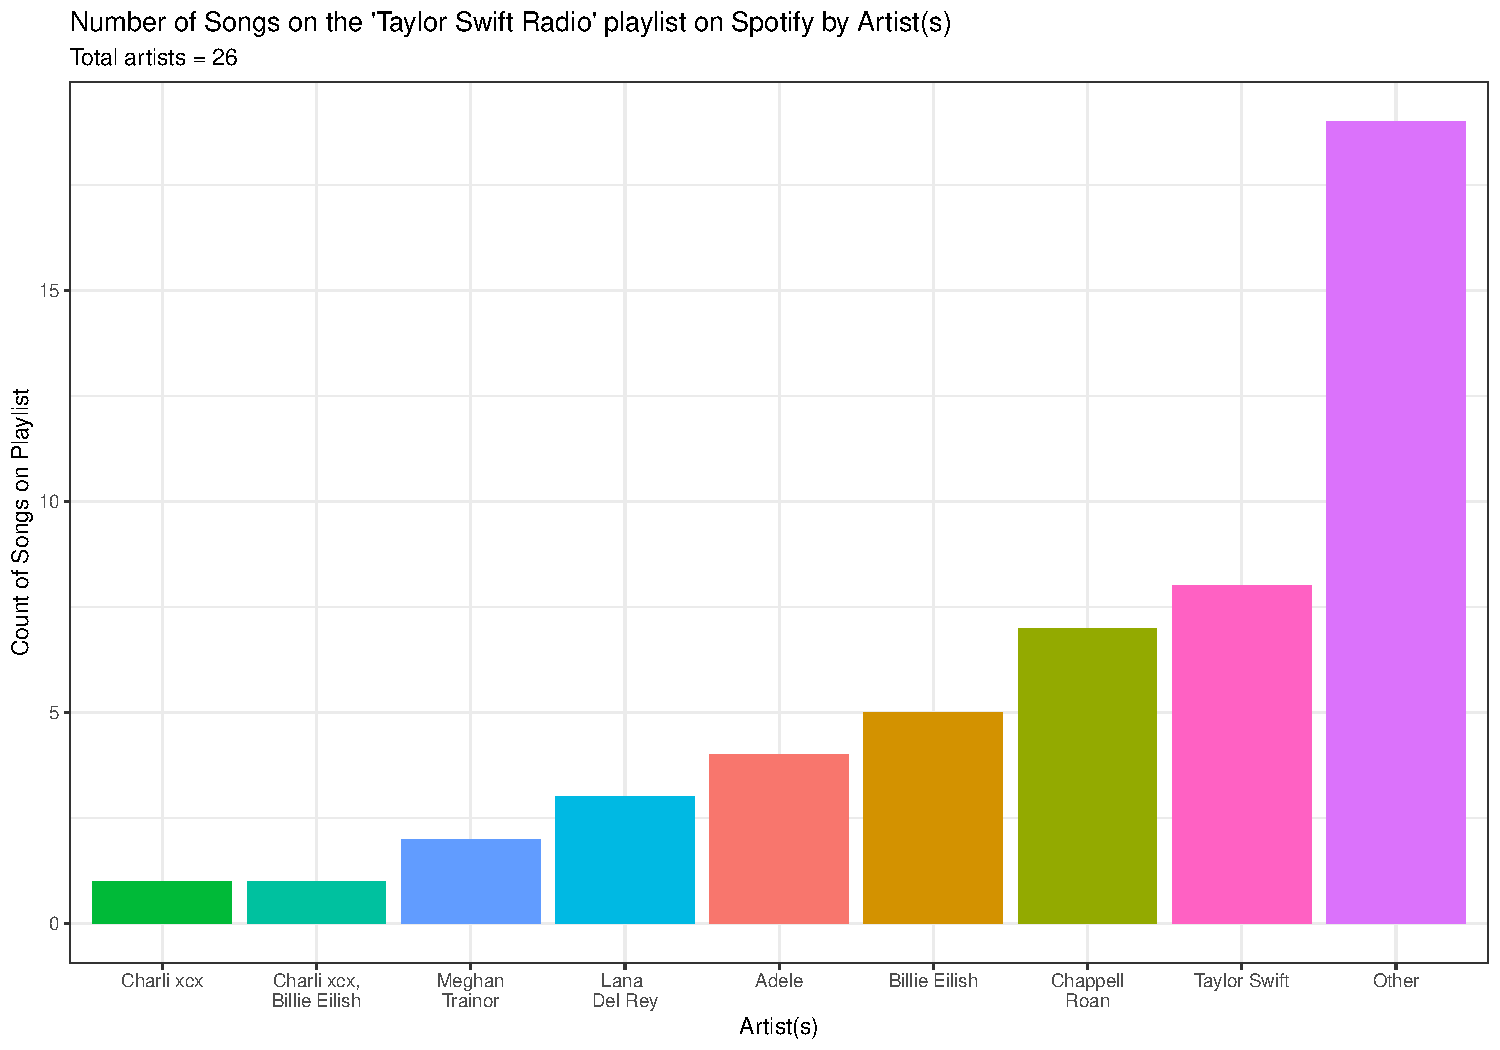
\includegraphics{class09_files/figure-beamer/unnamed-chunk-2-1.pdf}
\end{frame}

\begin{frame}{What if shuffle was truly random?}
\phantomsection\label{what-if-shuffle-was-truly-random}
Each time the song changes, every song on the playlist is eligible to be
played next

\begin{itemize}
\item
  Does not matter if the song was just played
\item
  Does not matter who the artist is
\end{itemize}

We call this \textbf{\emph{sampling with replacement}}.

\begin{itemize}
\item
  Like drawing a playing card, looking at it, then putting it back in
  the deck before the next draw
\item
  Repetition of outcomes is possible
\end{itemize}
\end{frame}

\begin{frame}{Sampling With Replacement}
\phantomsection\label{sampling-with-replacement}
\begin{center}
\includegraphics{class09_files/mediabag/Sampling-With-Replac.png}
\end{center}
\end{frame}

\begin{frame}{How often were artists repeated during Spotify's original
shuffle?}
\phantomsection\label{how-often-were-artists-repeated-during-spotifys-original-shuffle}
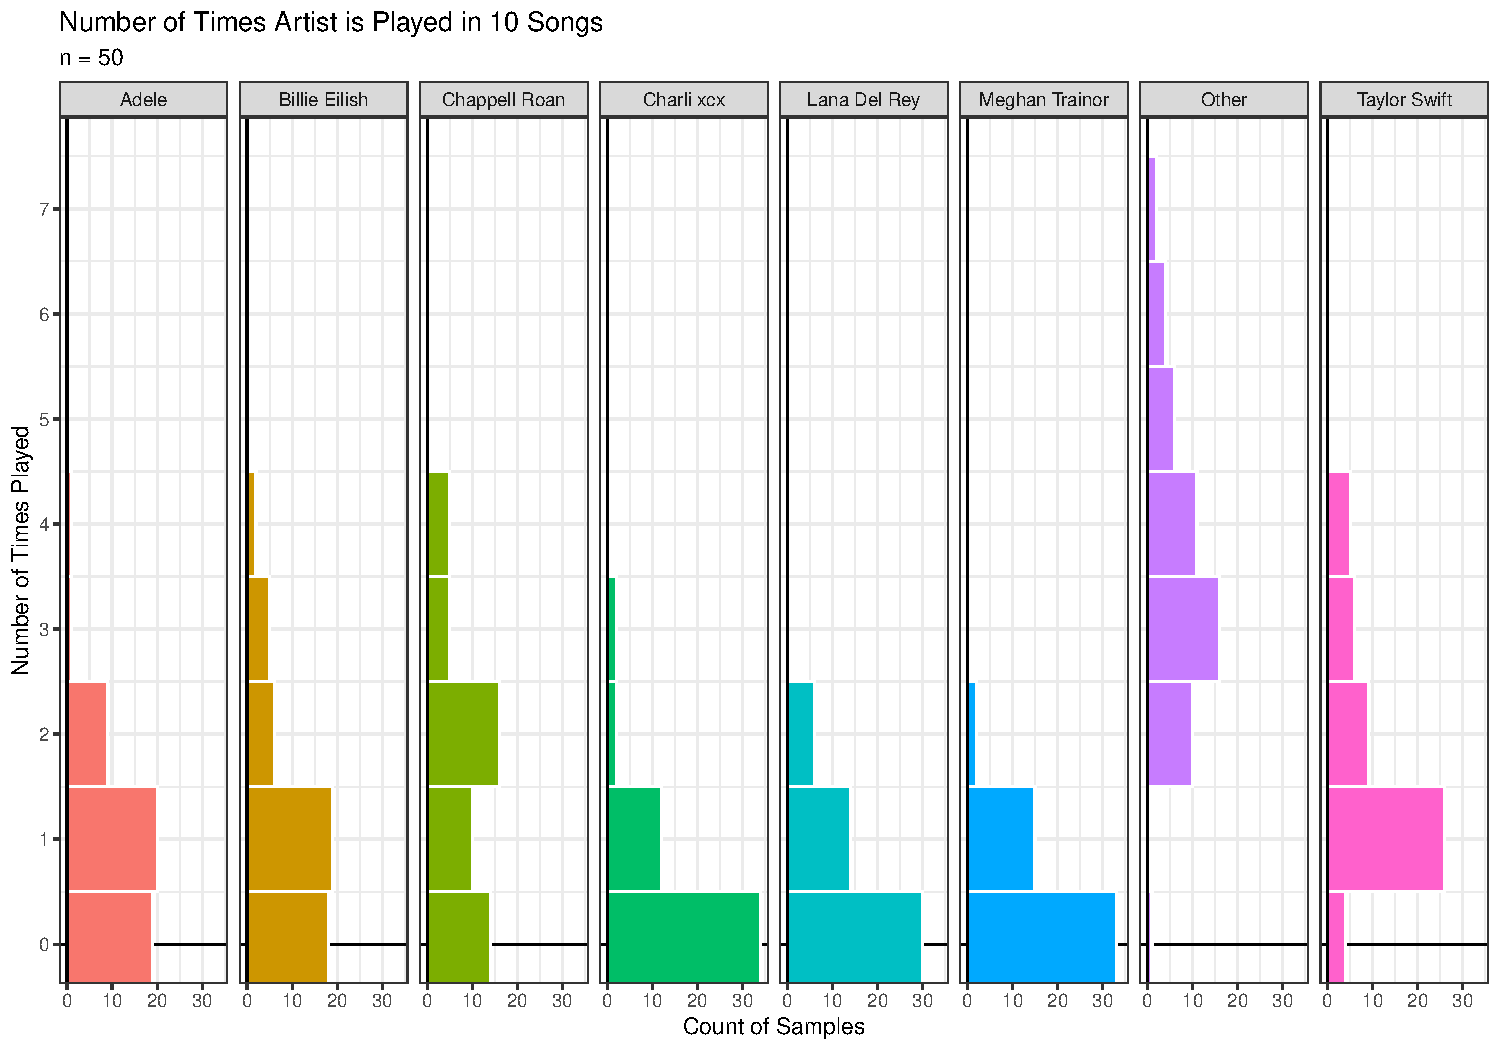
\includegraphics{class09_files/figure-beamer/unnamed-chunk-3-1.pdf}
\end{frame}

\begin{frame}{What is the probability of hearing a song by Chappell
Roan?}
\phantomsection\label{what-is-the-probability-of-hearing-a-song-by-chappell-roan}
\begin{itemize}
\item
  There is our ``observed'' probability that the next song is by
  Chappell Roan
\item
  Sample proportion (\(\hat{p}_n\))
\item
  There is some ``true'' real-world probability that the next song is by
  Chappell Roan
\item
  Population proportion (\(p\))
\end{itemize}
\end{frame}

\begin{frame}{Defining the sample space}
\phantomsection\label{defining-the-sample-space}
The \textbf{sample space} \(s\) or \(S\) is the total collection of
possible outcomes for a \textbf{random process}.

\begin{itemize}
\item
  Die rolls: 1, 2, 3, 4, 5, 6
\item
  Coin flips: heads, tails
\item
  Stock market: up, down, no change
\end{itemize}

Here, the \textbf{sample space} could be all the songs on the playlist
(n = 50) or all the artists who perform them (n = 26).
\end{frame}

\begin{frame}{Defining the Sample Space}
\phantomsection\label{defining-the-sample-space-1}
\begin{center}
\includegraphics{class09_files/mediabag/sample-space-example.png}
\end{center}
\end{frame}

\begin{frame}{Another sample space}
\phantomsection\label{another-sample-space}
\begin{center}
\includegraphics{class09_files/mediabag/card_ss.gif-raw=true}
\end{center}
\end{frame}

\begin{frame}{Disjoint Outcomes}
\phantomsection\label{disjoint-outcomes}
Outcomes are \textbf{disjoint} or \textbf{mutually exclusive} if they
cannot both happen at the same time

\begin{itemize}
\item
  Taylor Swift and Adele did not collaborate on any songs on this
  playlist
\item
  The next song played cannot be by both Taylor Swift and Chappell Roan
\item
  These are
\end{itemize}
\end{frame}

\begin{frame}{Non-Disjoint Outcomes}
\phantomsection\label{non-disjoint-outcomes}
\textbf{Non-disjoint} outcomes can occur at the same time.

\begin{itemize}
\tightlist
\item
  The next song played could be by Charlie xcx OR Billie Eilish, because
  they collaborated on a song
\end{itemize}
\end{frame}

\begin{frame}{Calculating probabilities}
\phantomsection\label{calculating-probabilities}
\begin{itemize}
\item
  Probabilities are proportions, or the number of observations with a
  particular value divided by\ldots{}
\item
  the total number of observations in a sample (\(n\))
\item
  the total number of outcomes in the sample space (\(s\))
\item
  Proportions range from 0 (no observations in data) to 1 (all
  observations in data)
\item
  Also may be a percentage, ranging from 0\% to 100\% (multiply
  proportion by 100)
\end{itemize}
\end{frame}

\begin{frame}{Proportion of Songs by Artist}
\phantomsection\label{proportion-of-songs-by-artist}
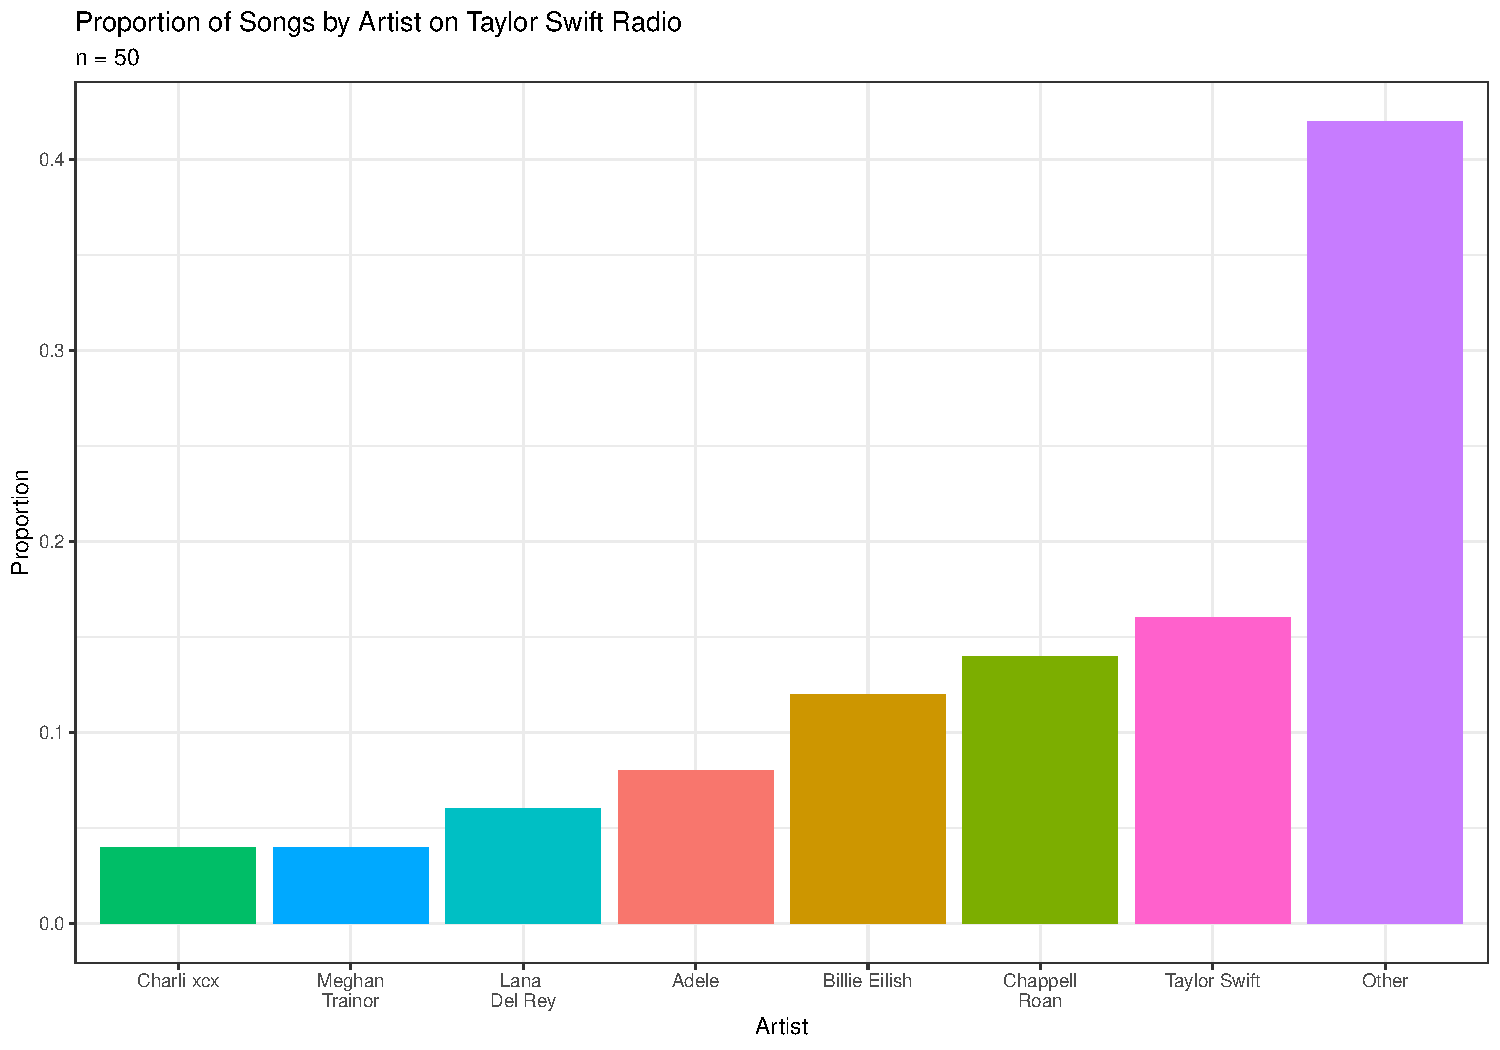
\includegraphics{class09_files/figure-beamer/unnamed-chunk-4-1.pdf}
\end{frame}

\begin{frame}{Proportion of Chappell Roan songs}
\phantomsection\label{proportion-of-chappell-roan-songs}
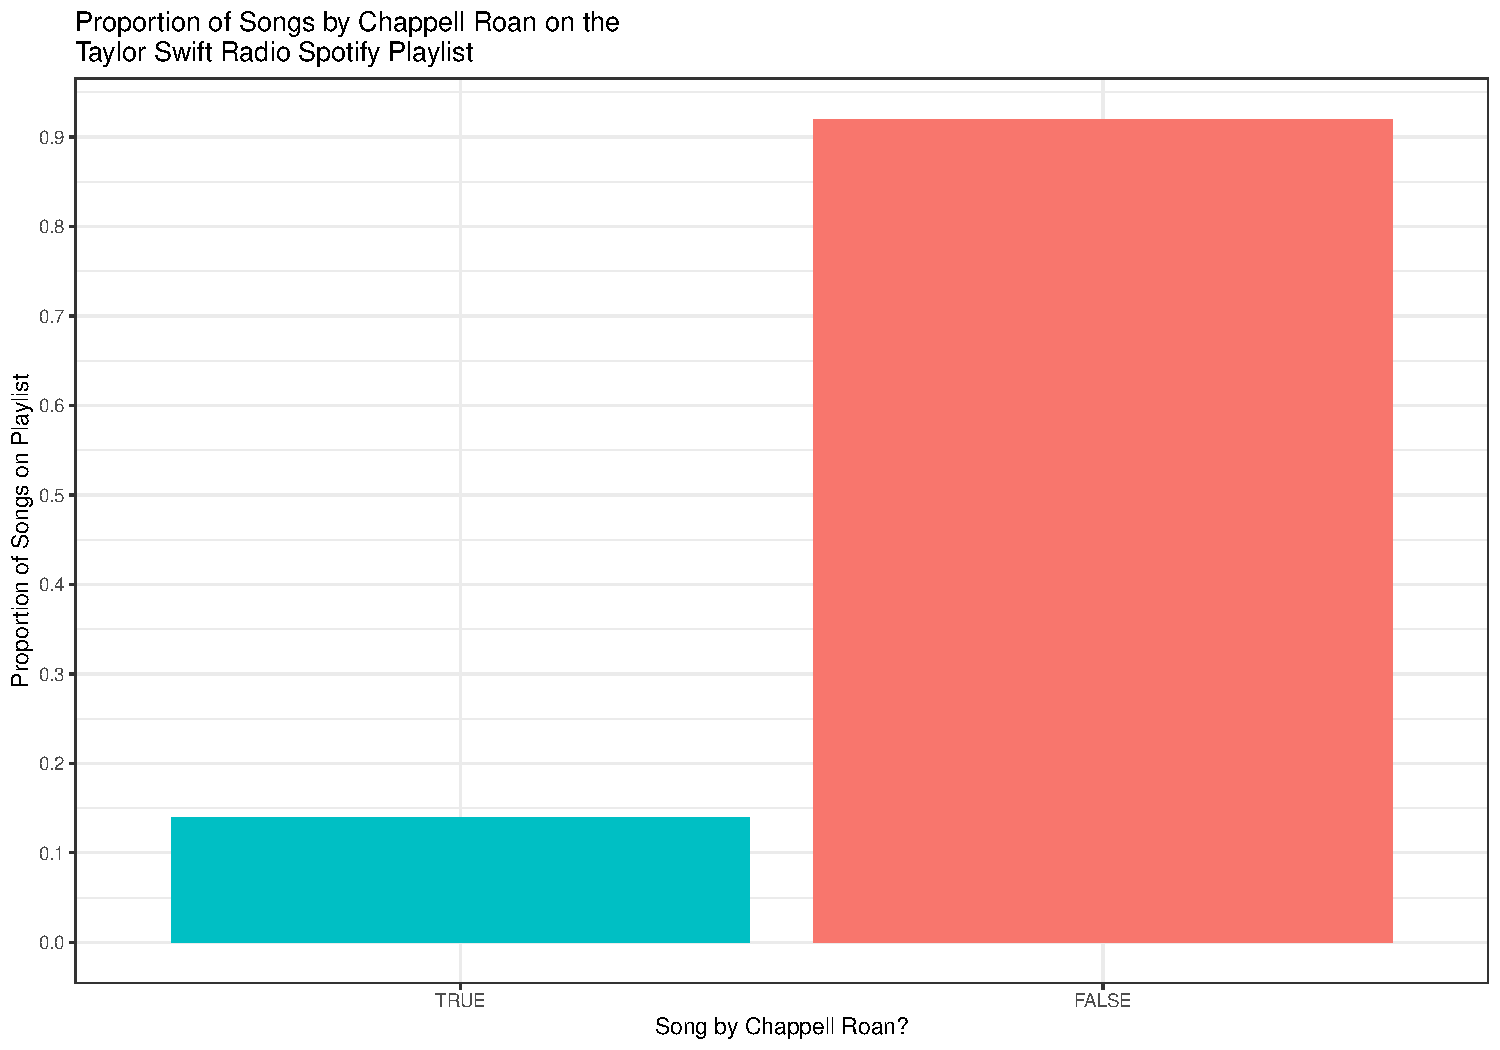
\includegraphics{class09_files/figure-beamer/unnamed-chunk-5-1.pdf}
\end{frame}

\begin{frame}{How well does a sample proportion represent the population
proportion?}
\phantomsection\label{how-well-does-a-sample-proportion-represent-the-population-proportion}
Should we listen to 1 song?

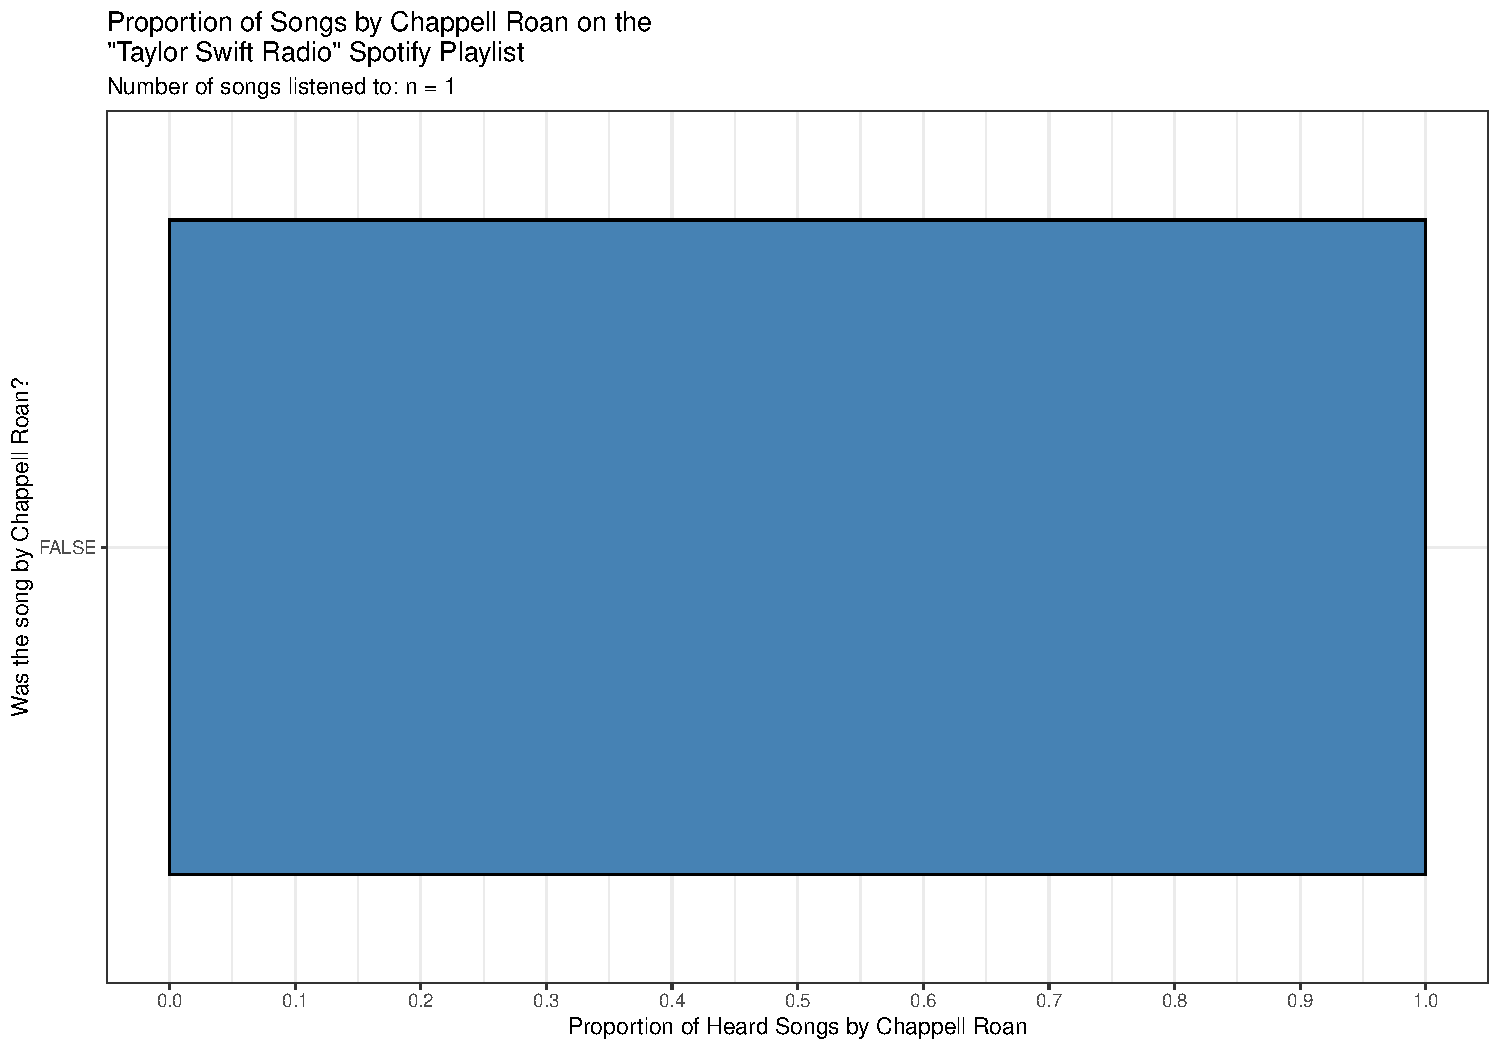
\includegraphics{class09_files/figure-beamer/unnamed-chunk-6-1.pdf}
\end{frame}

\begin{frame}{How well does the sample proportion represent the
population proportion?}
\phantomsection\label{how-well-does-the-sample-proportion-represent-the-population-proportion}
Should we listen to 5 songs?

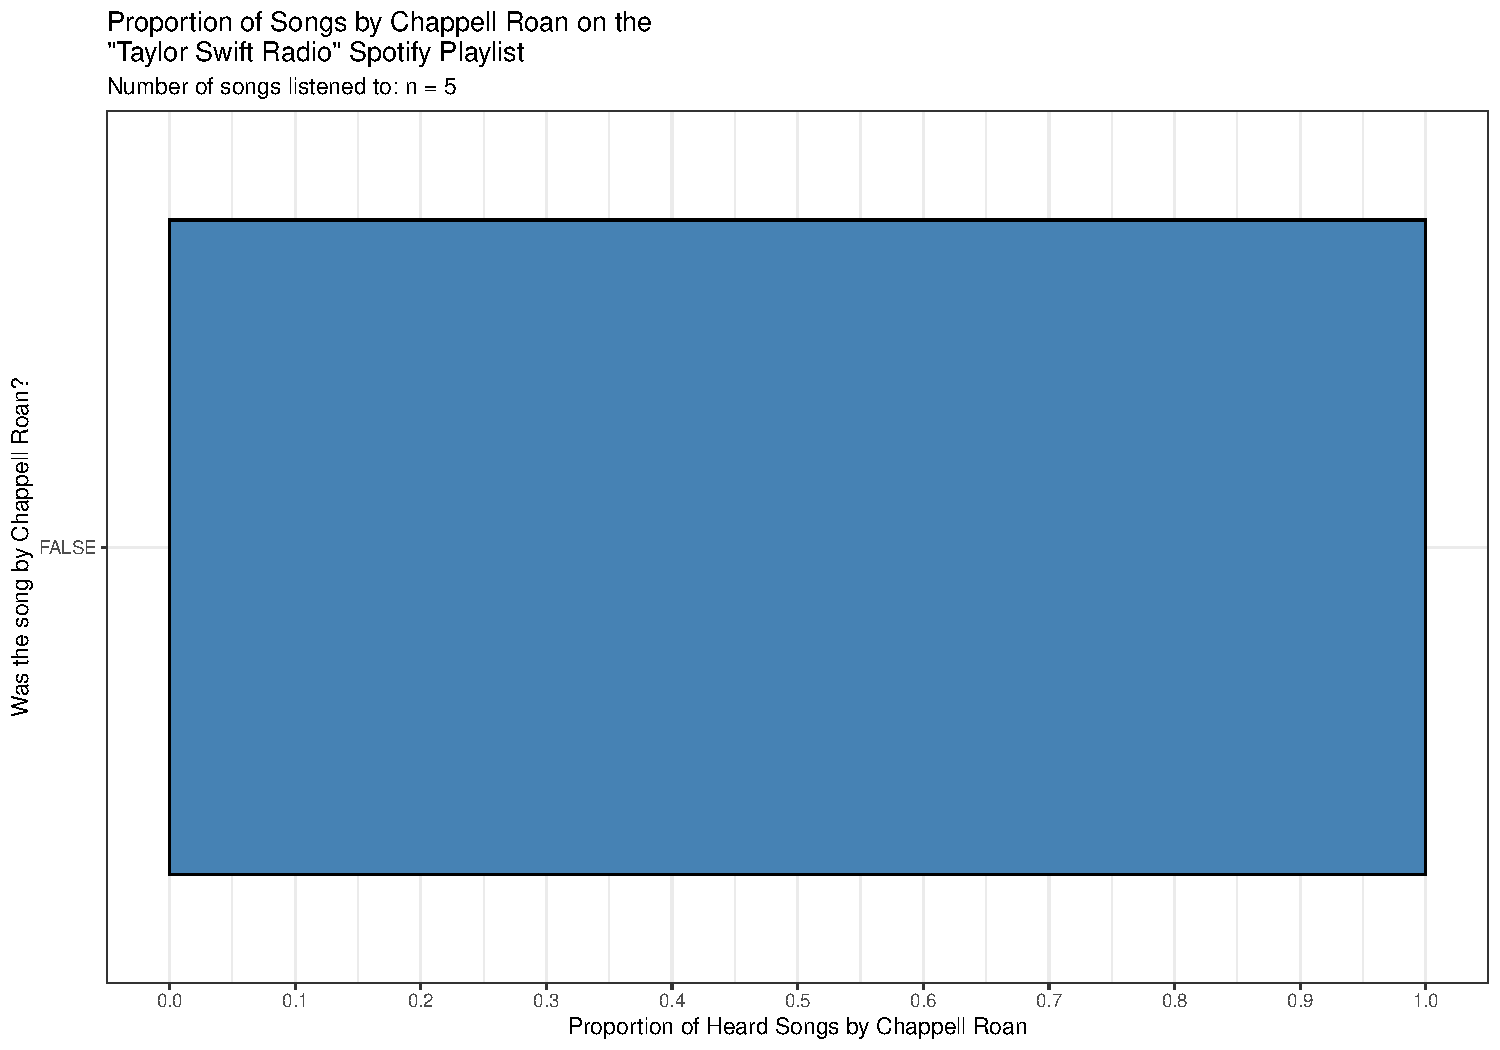
\includegraphics{class09_files/figure-beamer/unnamed-chunk-7-1.pdf}
\end{frame}

\begin{frame}{How well does the sample proportion represent the
population proportion?}
\phantomsection\label{how-well-does-the-sample-proportion-represent-the-population-proportion-1}
Should we listen to 10 songs?

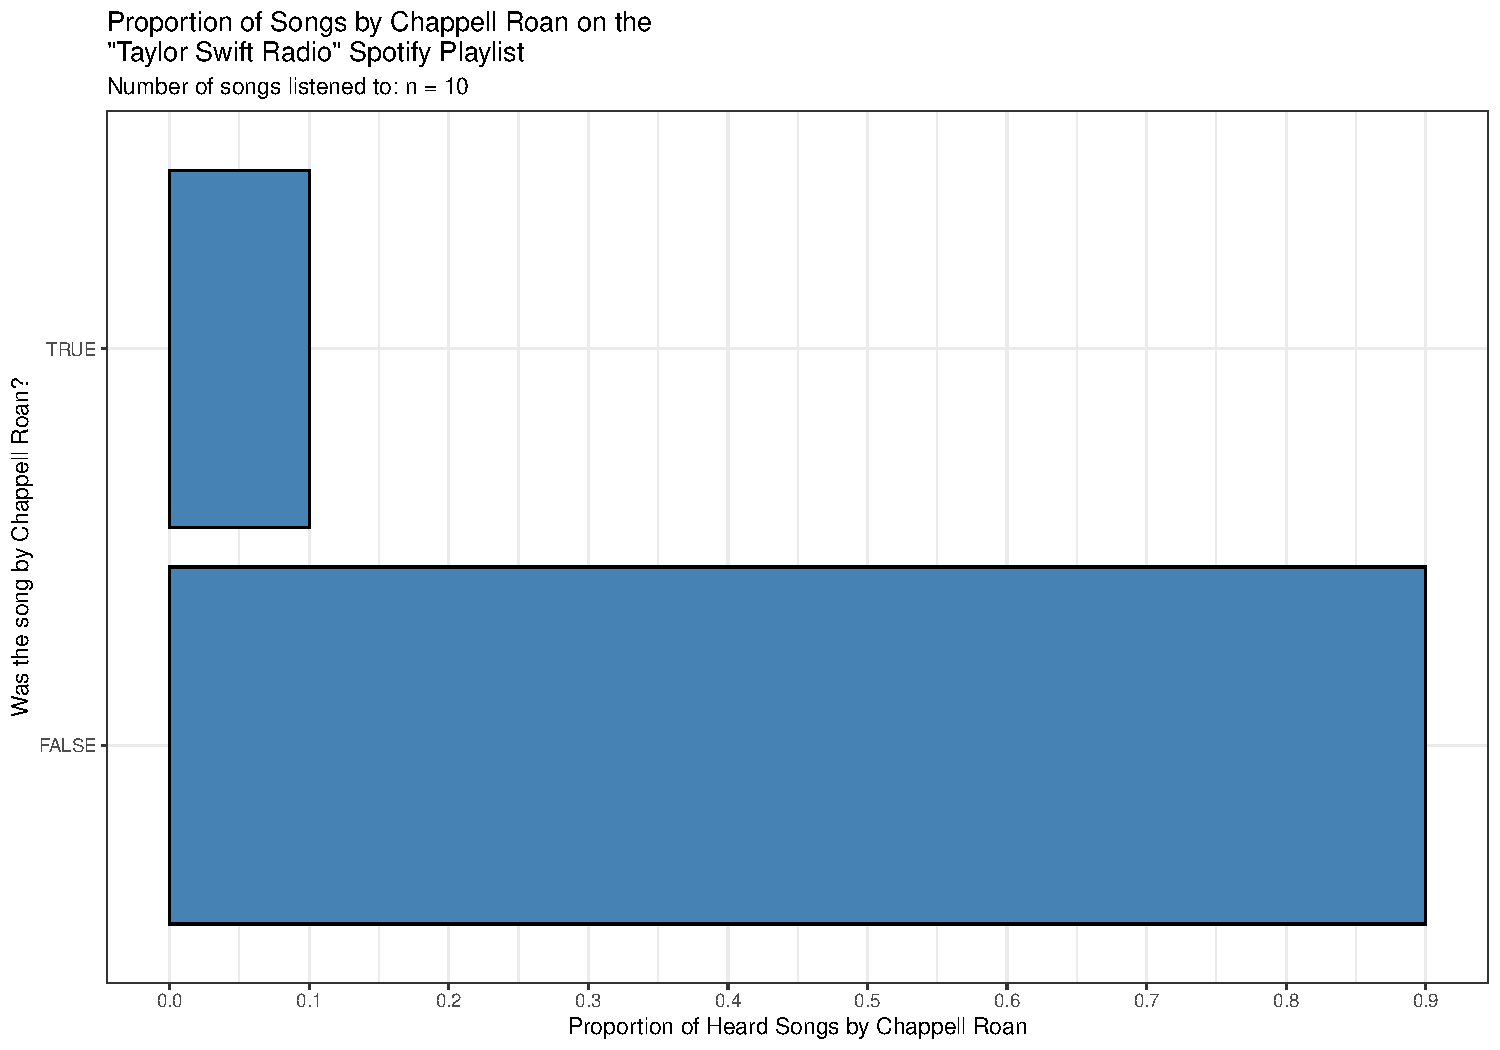
\includegraphics{class09_files/figure-beamer/unnamed-chunk-8-1.pdf}
\end{frame}

\begin{frame}{How well does the sample proportion represent the
population proportion?}
\phantomsection\label{how-well-does-the-sample-proportion-represent-the-population-proportion-2}
Should we listen to 100 songs?

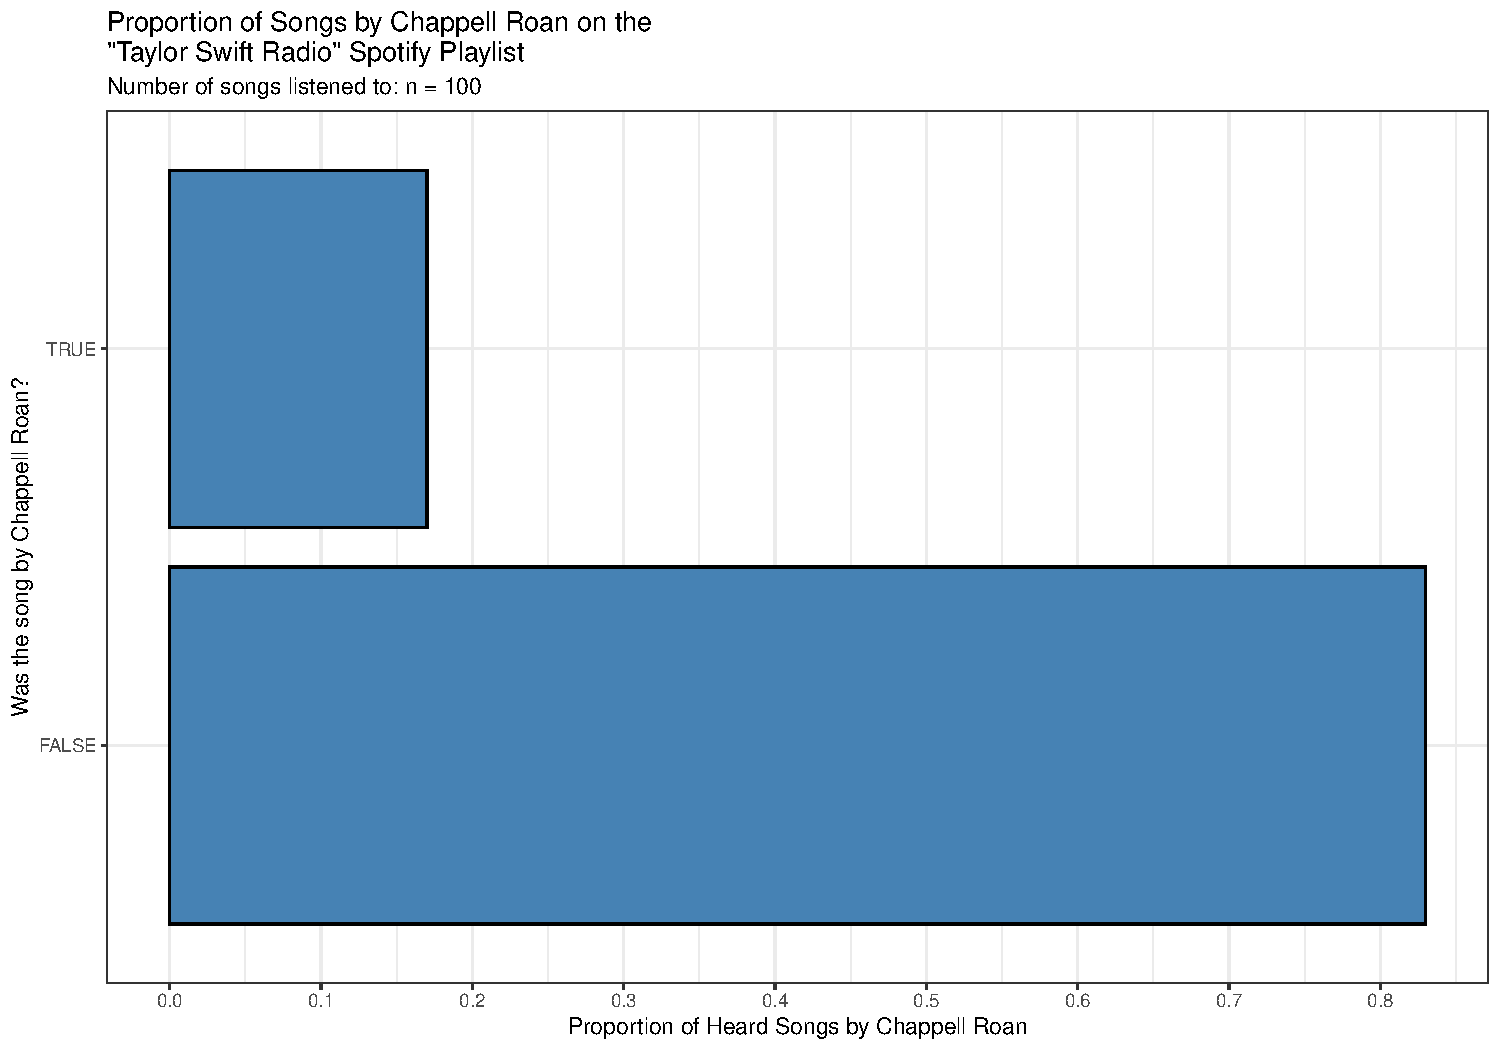
\includegraphics{class09_files/figure-beamer/unnamed-chunk-9-1.pdf}
\end{frame}

\begin{frame}{How well does the sample proportion represent the
population proportion?}
\phantomsection\label{how-well-does-the-sample-proportion-represent-the-population-proportion-3}
Should we listen to 200 songs?

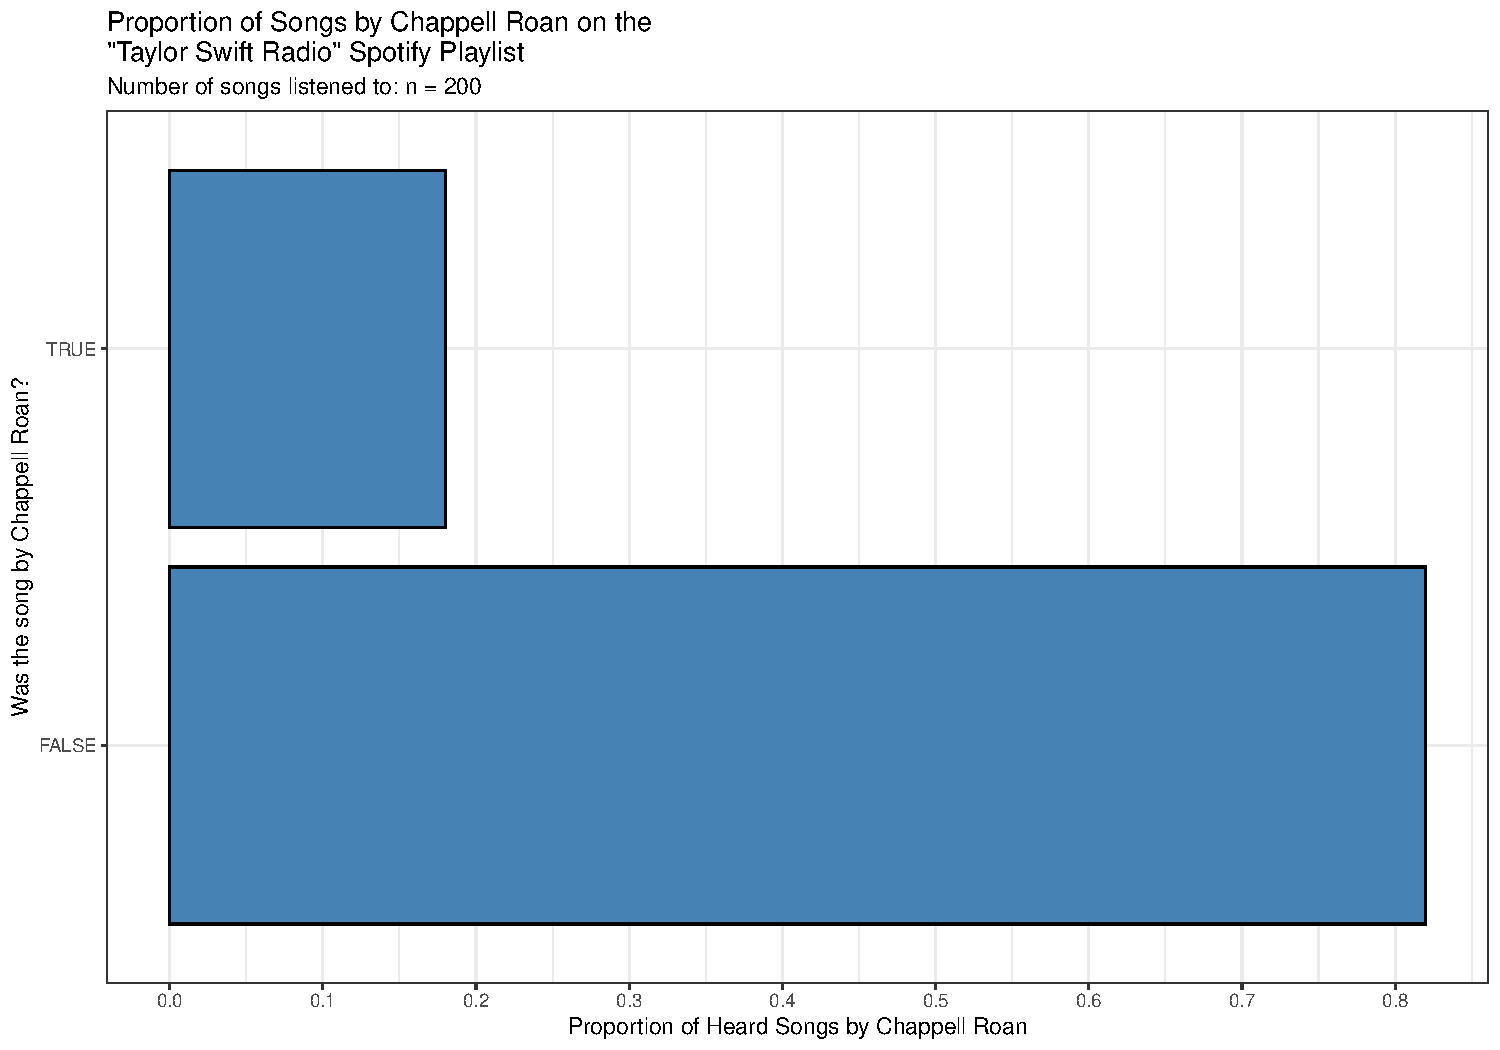
\includegraphics{class09_files/figure-beamer/unnamed-chunk-10-1.pdf}
\end{frame}

\begin{frame}{Law of Large Numbers}
\phantomsection\label{law-of-large-numbers}
As more observations are collected, the sample proportion \(\hat{p}_n\)
of a particular outcome approaches the population proportion \(p\) of
that outcome.

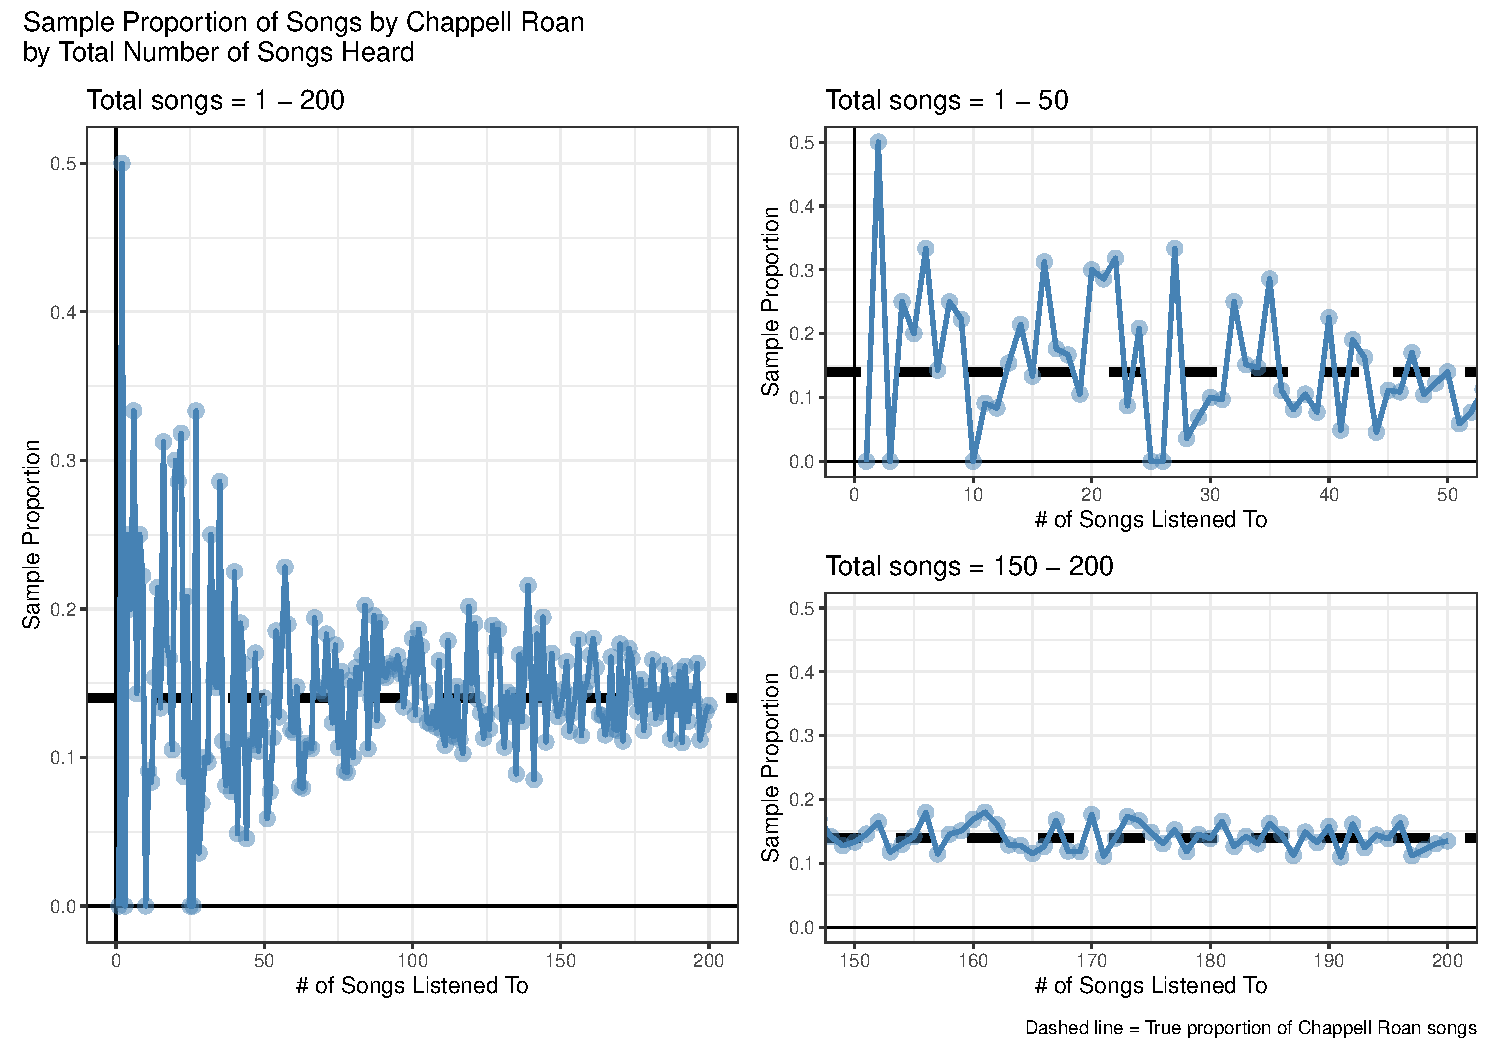
\includegraphics{class09_files/figure-beamer/unnamed-chunk-11-1.pdf}
\end{frame}



\end{document}
